%%%%%%%%%%%%%%%%%%%%%%%%%%%%%%%% 
\section{The Fine-Grained Tracker (FGT)} 
\label{cdrsec:detectors-nd-ref-fgt}

The scope of the DUNE Fine-Grained Tracker (FGT) near neutrino detector includes the design, procurement, fabrication, testing, delivery and installation of all the systems and components that comprise it:

\fixme{edit this as needed}

\begin{itemize}
\item a straw-tube tracking detector (STT)
\item electromagnetic calorimeter (ECAL) 
\item a 0.4-T dipole magnet surrounding the STT and ECAL
\item muon identifiers (MuIDs) ocated in the steel of the magnet, as well as upstream and downstream of the STT
\item instrumentation for monitoring and control
\end{itemize}



\begin{cdrfigure}[A schematic drawing of the fine-grained
tracker design]{STT_schematic}{A schematic drawing of the fine-grained tracker design.}
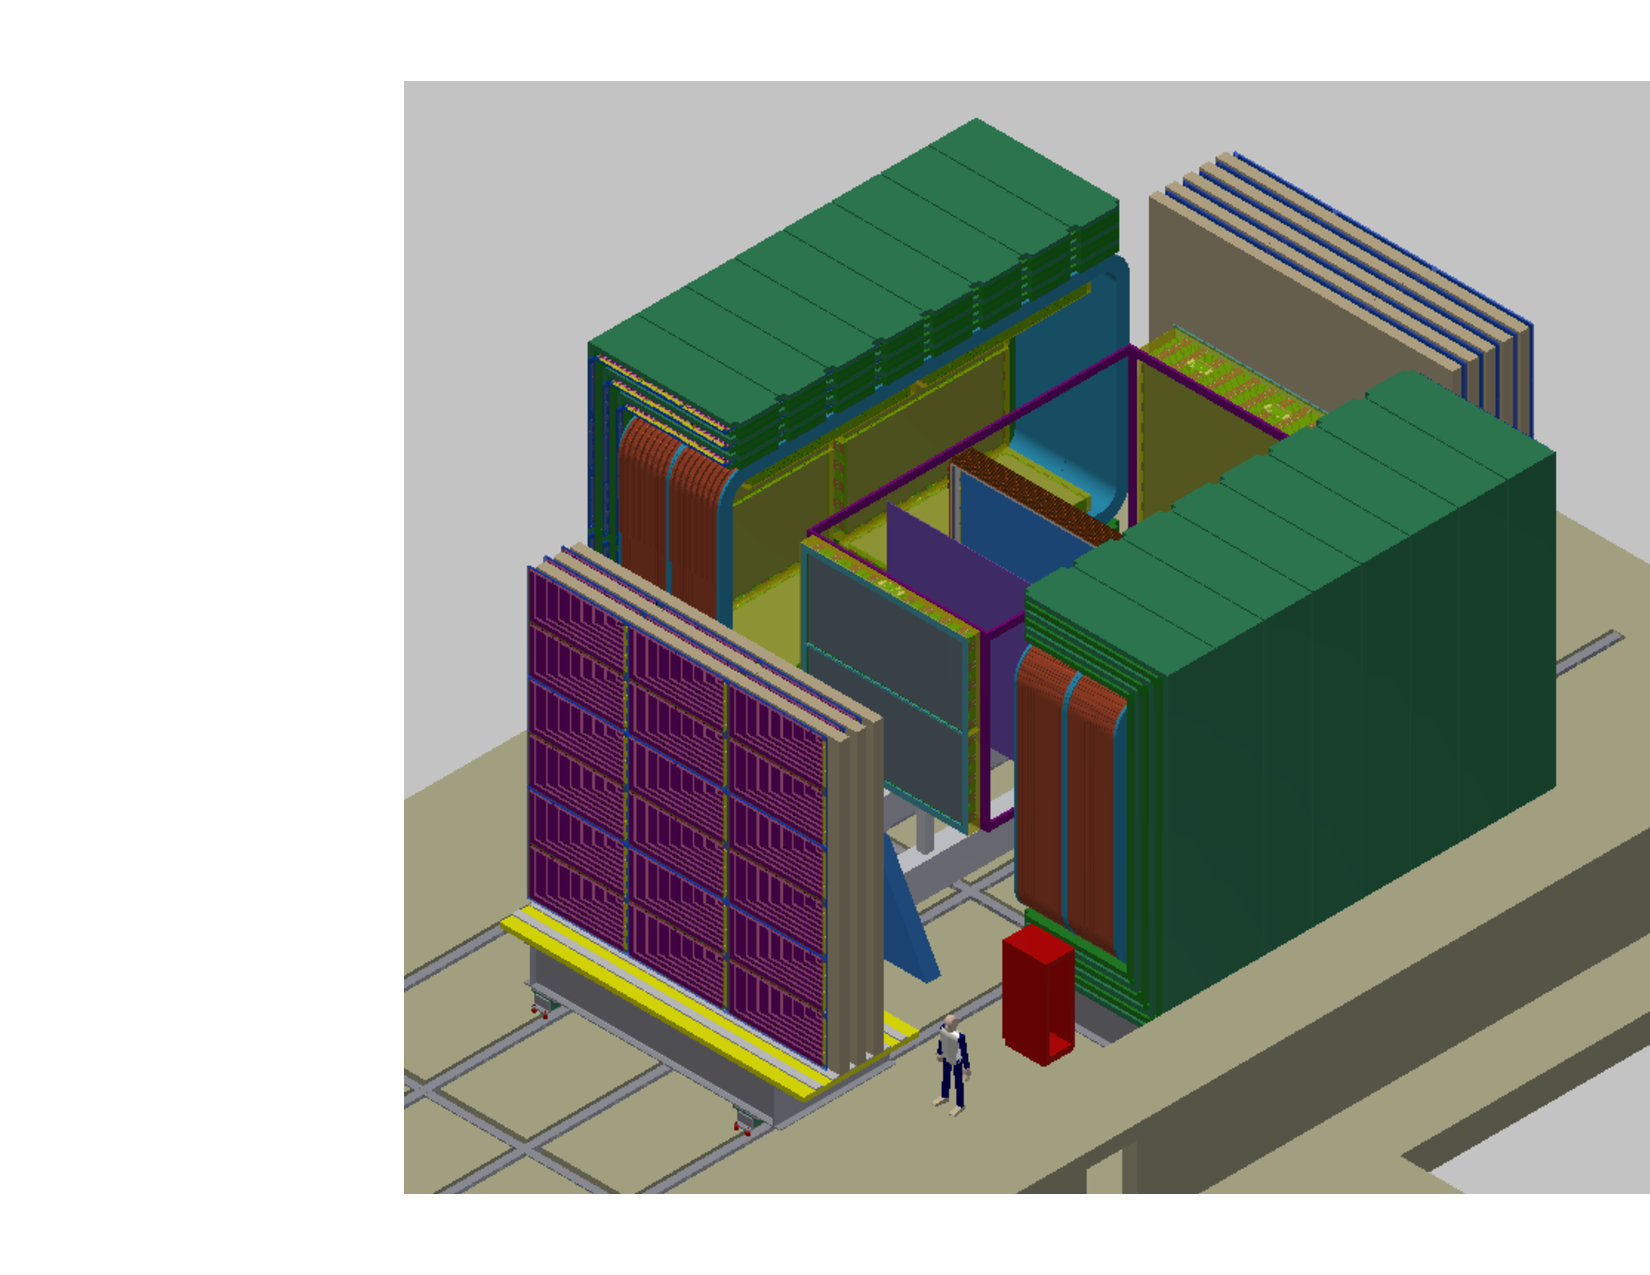
\includegraphics[width=\textwidth]{FGT_Overview}
\end{cdrfigure}

A schematic drawing of the FGT design is shown in Figure~\ref{fig:STT_schematic}.   The design presented here meets the required performance for making precision measurements of the 
neutrino fluxes, cross sections, signal rates and background rates for the DUNE far detector. The most significant requirements include 

\begin{itemize}
\item excellent position and angular resolutions
\item  identification and measurement of processes such as neutral current $\pi^0$ production that can mimic oscillation signals at the FD
\item comparability with measurements made in the FD
\item measurement of nuclear effects, including short-range correlations, two-body currents, pion absorption, initial-state interactions, 
and final-state interactions
\end{itemize}
Regardless of the process under study, the goal is
to have the systematic error less than the corresponding statistical error. A summary of the performance
requirements is given in Table~\ref{tab:comparison}

The FGT will measure the neutrino event rates and cross sections 
on argon, water, and other nuclear 
targets for both $\nu_e$ and $\nu_\mu$ charged current (CC) and
neutral current (NC) scattering events. The FGT design 
consists of a straw-tube tracker (STT), consisting of straw tubes, water targets, argon targets, 
and radiator targets, and an electromagnetic calorimeter (ECAL), both inside a
dipole magnet. In addition, muon detectors (MuID) consisting of resistive plate
chambers (RPCs) will be embedded in the steel
of the magnet. 

\begin{cdrtable}[A summary of the performance for 
the FGT configuration]{ll}{comparison}{A summary of the performance for 
the FGT configuration}
Performance Metric&FGT\\ \toprowrule
Straw Tube Detector Volume & 3.5m x 3.5m x 6.4m \\ \colhline
Straw Tube Detector Mass&8~t\\ \colhline
Vertex Resolution&0.1 mm \\ \colhline
Angular Resolution&2 mrad \\ \colhline
$E_e$ Resolution&5\% \\ \colhline
$E_\mu$ Resolution&5\% \\ \colhline
$\nu_\mu/\bar \nu_\mu$ ID&Yes \\ \colhline
$\nu_e/\bar \nu_e$ ID&Yes \\ \colhline
NC$\pi^0$/CCe Rejection&0.1\% \\ \colhline
NC$\gamma$/CCe Rejection&0.2\% \\ \colhline
CC$\mu$/CCe Rejection&0.01\% \\
\end{cdrtable}


%%%%%%%%%%%%%%%%% 
\subsection{Straw-Tube Tracking Detector}
\label{cdrsec:detectors-nd-ref-fgt-stt}

The Straw-Tube Tracking Detector (STT) at the center of the FGT
will be composed of straw tubes \fixme{made of what?} with an outer diameter of 1~cm, as well as 
radiators and targets that reside next to the straw tubes. %(see Figure~\ref{fig:STT_Detail}).
Vertical (YY) and horizontal (XX) planes of straws will be alternated and 
arranged in modules, with each module containing close-packed double straw layers 
of vertical and horizontal straws (XXYY). 
%Figure~\ref{fig:STT_Detail} shows a schematic drawing of an STT module with four straw-tube planes and
radiators. 

Radiators will be placed in the downstream STT modules
and will serve as targets for both neutrino interactions 
and Transition Radiation (TR) production. Each STT module contains 
four radiators, where each radiator consists of
60 layers of 25-$\mu$m polypropylene (C$_3$H$_6$)$_n$ 
foils alternating with 60 sheets of 125-$\mu$m tulle fabric spacers. 
The mass of each radiator is $\sim27$ kg and the thickness is 
$\sim9$ mm. 
Thin graphite planes and/or carbon fiber foils can be added to some STT modules
in order to have a total carbon target mass of about 0.5~t. (This is in addition to
the carbon in the STT frames.) A statistical subtraction of events occurring
on the pure carbon target from the ones in the polypropylene radiators will provide a measurement of
antineutrino interactions on a free proton target, which can be used for flux determination and cross
section measurements.

Both argon
and water will be implemented as target materials for neutrino interactions.
The targets will be 
positioned directly upstream of individual modules without radiators. 
The targets will consist of planes of 0.5-inch diameter, 3.5-m-long aluminum tubes filled
either with water (H$_2$O or D$_2$O) or with argon gas pressurized to 140 atm ($\rho = 0.233$).
Additional nuclear targets, such as Ca (same atomic weight as argon), C, stainless
steel, and Pb, can also be used in
the form of thin planes, to be positioned directly upstream of individual STT modules without radiators.



%%%%%%%%%%%%%%%%% 
\subsection{Electromagnetic Calorimeter}
\label{cdrsec:detectors-nd-ref-fgt-ecal}

An electromagnetic calorimeter 
(ECAL) will surround the tracking volume on all sides and consist of three separate pieces: Forward ECAL, Barrel ECAL, and Backward ECAL.  
The ECAL conceptual design consists of 
layers of either 1.75-mm-thick (for the forward ECAL) or 3.5-mm-thick 
(for the barrel and backward ECAL) lead sheets and 2.5-cm-wide by 10-mm-thick 
plastic scintillator bars.

The lead sheets and scintillator bars will be assembled and glued together
into complete modules of dimension 
3.2~m $\times$ 3.2~cm $\times$ 81~cm for the Forward ECAL and
3.2~m $\times$ 3.2~cm $\times$ 27.5~cm for the Backward ECAL. For the Barrel ECAL, the module 
dimensions will also be 
3.2~m $\times$ 3.2~cm $\times$ 27.5~cm. Two Barrel modules are placed end-to-end 
along the sides of the inner surface of the magnet (eight Barrel modules
total) to provide full coverage of the barrel region.

The scintillator bars will be extruded with 
holes in the middle of each bar. The
holes will then be fitted with 0.7-mm-diameter Kuraray wavelength-shifting (WLS) fibers.
The fibers will be read out by SiPM (silicon photomultiplier) photosensors at each end.

%%%%%%%%%%%%%%%%% 
\subsection{Dipole Magnet}
\label{cdrsec:detectors-nd-ref-fgt-magnet}

The STT and ECAL modules will reside inside a 0.4-T dipole 
magnet for the measurement of particle momentum and charge. 
The magnet will have inner dimensions (inside the coils) 
4.5-m wide $\times$ 4.5-m high $\times$ 8.0-m long. The 
magnet has four vertical Al coils, stacked horizontally, producing a horizontal magnetic 
field. The return yoke will be divided into two halves along the 
longitudinal center line to allow the magnet to be opened to service the
detector inside. %, as shown in Figure~\ref{fig:STT_schematic}. 
Each half yoke will be built
from eight ``C'' (C-shaped) sections, and the thickness of the 
magnet steel will be 60~cm, consisting of 6
$\times$ 10-cm-thick plates. The magnet power requirement with Al coils is $\sim 2.4$~MW,
corresponding to 6~kA at 400~V. The water flow required for cooling is 20~l/s.

The momentum resolution is dominated by multiple scattering in the STT. The momentum resolution is, therefore, given by 
$\delta p/p = 0.053/\sqrt(LX_0)B$. For B = 0.4T, L = 3m, and $X_0 = 4$m, the
expected momentum resolution is $\sim 3.8\%$. 

%%%%%%%%%%%%%%%%% 
\subsection{Muon Identifier}
\label{cdrsec:detectors-nd-ref-fgt-muonid}

The sides and ends of the dipole magnet will be instrumented
with a muon identifier
detector (MuID) that will distinguish muons from hadrons by the ability 
of muons to penetrate the iron without showering or interacting.
The MuID will consist of 432 resistive plate chamber (RPC) modules
interspersed between two 10-cm-thick steel plates of the 
dipole magnet and between 20-cm-thick steel plates at the upstream and
downstream ends of the magnet. 
The MuID is only meant to provide %the 
identification of the 
muon; the muon momentum %itself 
will be measured by the STT inside the 
magnetic field.

%%%%%%%%%%%%%%%%% 
\subsection{Instrumentation}
\label{cdrsec:detectors-nd-ref-fgt-instrum}

The instrumentation includes both fast readout electronics for the subdetectors
and the slow control ($\mathcal{O}$ seconds) of the subdetectors, involving monitoring the humidity, 
temperature, gas pressure, etc.
There is considerable synergy in the information gathered in the STT, ECAL and MuID. 
Both the STT and ECAL are required to measure the total charge and the time associated with a 
given hit. The MuID RPCs are required to provide the position and time associated with 
a traversing track. Similarly, the slow control of the subdetectors
share many features.

The electronics for the three subsystems, STT, MuID, and ECAL, are all ``fast'' systems, 
i.e., all of the signals are in the few-to-10 nanosecond range. 
The requirements for each system are very similar: a fast output and both an ADC  
and a TDC on each channel.  Additionally, for the STT straw tubes it 
is desirable to wave-form digitize the analog signal in order to enhance the ability to separate 
the ionization signal from the transition radiation signal. 

Recently, an interesting new ASIC development for an upgrade to the ATLAS muon system at the LHC
has come out of BNL), the VMM2 chip. %\fixme{add G. DeGeronimo at BNL ref} 
 It handles 64 channels and produces both fast ADC and TDC outputs.
It has been fabricated and tested and should be ready by 2017, long before it will be needed for DUNE.

To maintain a low level of 
humidity and to maintain a desired temperature, both STT and ECAL subdetectors
will have dry nitrogen circulating within their outer layers.  Magnet coils are cooled by water, 
while the magnet yokes are instrumented with RPCs that must remain dry. Continuous control of 
humidity in all these detectors is needed.
Temperature must also be continuously monitored in all of the subdetectors
in order for the electronics to not overheat. 
To ensure that the magnet does not overheat, the water flow (pressure gradient) will be continuously monitored.  
Also, all power sources instrumenting the FGT and its readout need to be monitored for 
appropriate voltage and current.


